\documentclass[11pt]{article}
\usepackage[review]{vendor/acl}
\usepackage{times}
\usepackage{latexsym}
\usepackage[T1]{fontenc}
\usepackage[utf8]{inputenc}
\usepackage{microtype}
\usepackage{inconsolata}
\usepackage{booktabs}
\usepackage{graphicx}
\usepackage{tikz}
\usetikzlibrary{arrows.meta,positioning}
\title{ScreenshotLegalBench: Evidence-Grounded Understanding and Reconstruction of Chat Screenshots}
\author{Anonymous authors}
\date{}

\begin{document}
\maketitle
\begin{abstract}
Chat screenshots used in legal work require more than optical character recognition: an analysis must associate speakers and statements, preserve uncertain time information, relate multiple conversations, and identify the visual source of every material claim. We present a working research protocol for renewing ScreenshotLegalBench, starting from an audited collection of 1,170 image files and existing screenshot classification, message extraction questions, and multi-image cause-of-action questions. We distinguish reproducibility work on the legacy benchmark from a proposed extension to event reconstruction and complementary evidence submitted by opposing parties. The extension uses judgment-constrained synthetic conversations, explicit generation provenance, and questions with verified evidence dependencies. We define evaluation controls for failure denominators, human legal grading, case-family isolation, and evidence removal. This manuscript reports an asset audit and offline baselines. A 24-question model pilot is available; full comparisons and reconstruction experiments remain pending. It makes no claim of improved model performance or demonstrated benchmark difficulty.
\end{abstract}

\section{Introduction}
Legal practitioners often receive fragmented screenshots rather than a complete conversation export. A useful system must identify who made a statement, what it expressed, when it occurred, and which screenshot region supports that interpretation. Multiple screenshots may overlap; distinct conversations may concern the same event; apparent chronology can remain underdetermined. In a two-party evidence setting, the submitted materials can be complementary or conflicting. A system should reconstruct the observable record and expose gaps rather than invent missing messages.

The existing ScreenshotLegalBench project studies key information extraction (KIE) and visual question answering (VQA) in chat screenshots. Its public repository also records the addition of closed-source model experiments during rebuttal \citep{screenshotlegacy}. Renewing this research requires recovering exact datasets and evaluation protocols before extending its claims. Historical manuscript statistics, annotation snapshots, and evaluation tables do not always share a denominator.

This working manuscript separates two stages. Version 1 evaluates existing tasks using fixed contemporary vision-model endpoints, selects a model using task-specific and evidence-grounding criteria, and then validates an evidence organization application. Version 2 audits question quality and develops judgment-constrained synthetic cases with known messages, events, and screenshot coordinates. The stages form a development feedback loop, while published evaluation sets remain frozen.

The intended research question is: \emph{where do visual extraction, evidence association, and legal interpretation fail, and does an evidence-grounded event representation improve cross-screenshot understanding?} The asset audit and task adapter are implemented. The event tasks, full model comparison, and application validation remain proposed. This distinction is essential to interpret every table and claim below.

\section{Scope and Relation to Prior Work}
Legal judgment analysis can couple facts with retrieved legal premises rather than merely predicting an outcome \citep{deng2023}. Our focus begins earlier in the workflow, with visual evidence and its provenance. A judgment is an offline source for constructing a research sample, not information available to a model answering a screenshot-only test question. Judgment holdings must not leak into inference prompts.

We borrow the modular workflow contract from LegoFlow \citep{legoflow2026}: stages own their configuration, scripts, skills, dependencies, and artifacts, and communicate through explicit intermediate objects. Its software-engineering task collection and executable rewards are domain specific. They do not provide a correctness oracle for legal evidence. In this project, validated rendering can provide message coordinates and ordering truth, but legal interpretations still require independent expert review.

This draft does not establish priority over all legal multimodal benchmarks or claim to be the first of its kind. A systematic related-work comparison and recovery of the submitted manuscript are required before preparing a submission. The local file named \texttt{2023.emnlp-main.864.pdf} is the reference paper by \citet{deng2023}, not a version of the ScreenshotLegalBench manuscript.

\section{Asset Audit and Legacy Tasks}
\subsection{Images, Records, and Cases}
The audited image index contains 1,088 images from the main evaluation directory and 82 additional images resolved from the human-answer collection. All 1,170 indexed files passed image verification. The index contains 313 filename-prefix groups, of which 225 contain multiple images. These groups are provisional identifiers, not independently verified judicial cases. Two groups of identical image hashes require annotation-aware review.

The legacy classification annotation contains 1,176 records, including repeated classification records for six image filenames. The current adapter preserves their historical weighting. Any deduplicated evaluation must receive a new dataset version. Existing multi-image cause-of-action questions have 154 complete image inputs. Neither the 154 question groups nor the 225 multi-image filename groups implies that every question requires multi-hop reasoning.

\begin{table}[t]
\centering
\small
\begin{tabular}{lr}
\toprule
Input protocol & Task records \\
\midrule
Screenshot classification & 1,176 \\
Evidence-form classification & 1,174 \\
Private/group chat classification & 1,174 \\
Single-image open case analysis & 1,174 \\
Multi-image open case analysis & 154 \\
Multi-image cause-of-action selection & 154 \\
Assisted message questions & 6,333 \\
Image-grounded message questions & 6,333 \\
\bottomrule
\end{tabular}
\caption{Frozen legacy task inputs. Protocols share images and labels; their sum is not a count of independent new examples. The image-grounded message protocol is an adapter over unchanged legacy questions and answers.}
\label{tab:tasks}
\end{table}

\subsection{Input Protocols and Annotation Limits}
Assisted message prompts include historical model-derived text. The image-grounded protocol supplies only the requested field and manually annotated image region. They must be reported separately. Of 6,333 historical message questions, 1,475 passed the recorded extraction IoU check and 4,858 did not. This diagnostic concerns a previous extraction pipeline; it does not justify dropping the latter questions from a full-denominator evaluation.

Historical KIE experiments refer to 143 images and 696 messages. The exact test snapshot has not been recovered locally and cannot be assumed equal to the current 450 structured-image records. Older classification distributions also differ from the current snapshot. We therefore avoid reproducing manuscript tables from incompatible files.

\subsection{Human Scoring Assets}
Archived exports contain generation prompts, grading prompts, expert scores, and error examples. One generation-scoring sheet has 351 data rows and 337 distinct case identifiers. Four human-score columns contain 175, 175, 191, and 175 nonempty entries. Three observed columns use scores within 0--4, while the fourth includes 5. These observations require recovery of rubric versions and paired sample identities before agreement estimation. A correlation computed on incompatible scales or unmatched samples would not establish scoring validity.

Historical error annotations include timestamp misreading, speaker attribution, content hallucination and omission, entity attribution, title recognition, and meme recognition. We propose extending this taxonomy with cross-conversation identity errors, unsupported events, temporal contradictions, and incorrect evidence-page citations. The extensions are proposed categories, not measured historical error frequencies.

\section{Evidence Representation and Application}
\subsection{Source-Grounded Messages and Events}
Each input image records a stable identifier, SHA256, evidence page, submitting party, and conversation identifier. A message preserves visible text, local speaker identity, normalized identity when supported, raw time text, normalized time or interval, precision, and a bounding box. Uncertain identity matches remain explicit candidates rather than forced merges.

An event groups material expressions and supporting messages. A source reference contains an image identifier, evidence page, message identifier, bounding box, and visible quotation. Multiple source references are retained when an event spans screenshots. A timestamp inferred from context must remain distinguishable from a visible timestamp. Missing years and relative-date labels require an interval or an unknown value when the capture date is unavailable.

\subsection{Judge and Lawyer Views}
In the judge view, images submitted by both parties are aligned to identify observable overlap, complementary messages, gaps, and conflicts. Overlapping submissions remain traceable to both origins. The output is a reconstruction of supported content, not a claim to recover unsubmitted text.

In the lawyer view, favorable, adverse, and neutral assessments are relative to a specified client and legal issue. Assessments include a rationale and source references. Working-view selection and export choices remain separate from the preserved original materials and complete extracted record. Both modes require professional review of legal significance.

Internal retrieval operates over speakers, time, messages, events, and quotations and returns the evidence source. Retrieval of analogous decisions and applicable provisions uses a separate adapter with source and version metadata. It is not silently replaced by keyword search over screenshots. Excel exports must include time, speaker, material expression, quotation, evidence pages, and sentence-level source references; the same reviewed rows support a timeline presentation.

\begin{figure*}[t]
\centering
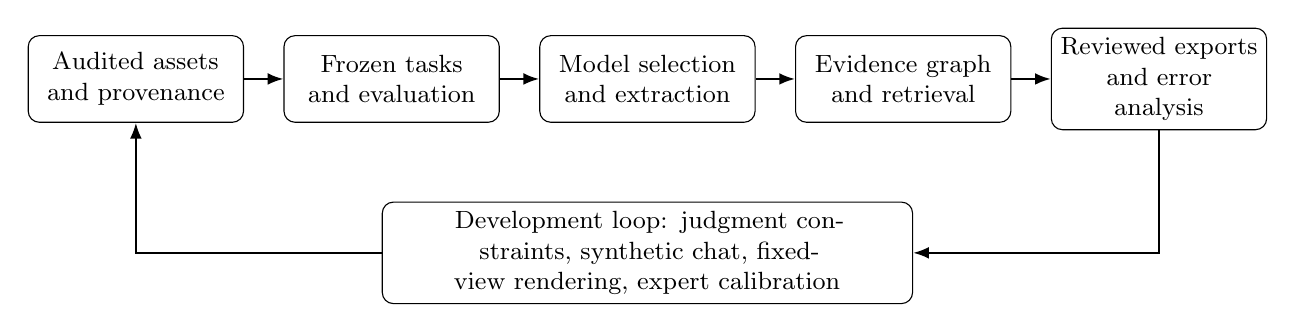
\begin{tikzpicture}[node distance=5mm and 5mm,
  box/.style={draw,rounded corners,align=center,font=\small,text width=25mm,minimum height=11mm},
  arrow/.style={-{Latex[length=2mm]},thick}]
\node[box] (a) {Audited assets\\and provenance};
\node[box,right=of a] (b) {Frozen tasks\\and evaluation};
\node[box,right=of b] (c) {Model selection\\and extraction};
\node[box,right=of c] (d) {Evidence graph\\and retrieval};
\node[box,right=of d] (e) {Reviewed exports\\and error analysis};
\draw[arrow] (a)--(b); \draw[arrow] (b)--(c);
\draw[arrow] (c)--(d); \draw[arrow] (d)--(e);
\node[box,below=10mm of c,text width=65mm] (f) {Development loop: judgment constraints, synthetic chat, fixed-view rendering, expert calibration};
\draw[arrow] (e.south) |- (f.east);
\draw[arrow] (f.west) -| (a.south);
\end{tikzpicture}
\caption{Target workflow inspired by modular block contracts. Asset indexing and offline input validation are complete. Full model evaluation, evidence software, and the synthetic extension remain pending. Development feedback must not optimize against a frozen test set.}
\label{fig:workflow}
\end{figure*}

\section{Judgment-Constrained Synthetic Extension}
\subsection{Generation Provenance}
Real screenshot authorization is difficult to obtain. The proposed extension starts from judgments with documented reuse conditions and retained source positions. Each generated message receives one provenance label: verbatim judgment quotation, judgment paraphrase, or synthetic completion. Exact quoted chat text is locked; paraphrases supply constraints; synthetic additions must not contradict those constraints. None of the generated samples is presented as authentic litigant evidence.

Chinese judgments produce WeChat-style interfaces and English judgments produce WhatsApp-style interfaces. Language, platform, and jurisdiction are recorded separately. A platform or language change must not silently change applicable law. Naturalistic dialogue and legal-fact fidelity are distinct quality axes, and a fluent chat does not compensate for an invented legally material fact.

\subsection{Rendering and Evidence Dependencies}
A structured conversation is rendered through a frontend with a fixed viewport, recorded fonts, scaling, layout version, and random seed. The renderer records message-to-image mappings and bounding boxes. Controlled crops, overlaps, and party-specific views create reconstruction tasks with observable reference truth. Layout and visual degradation variations are evaluated separately from semantic changes.

Each question includes a reviewed answer, a minimal sufficient evidence set, and an explicit dependency graph when multi-hop reasoning is claimed. Removing a necessary image should make the task unanswerable or change the supported answer; removing irrelevant images should leave it stable. Text-only and single-image controls test whether titles, templates, options, or incidental metadata reveal the answer.

\subsection{Quality Loop and Isolation}
Development failures inform candidate generation and prompt changes. A calibration set supports grading-prompt selection; a frozen test set is withheld from those decisions. The same judgment, derived chats, screenshot chains, and near-duplicate variants belong to one split. A release records judgment-family overlap checks and contamination limits. The system may improve candidate generation or retrieval without model training; fine-tuning is optional and requires a separate verified benefit.

\section{Evaluation Protocol}
Every inference run binds the dataset digest, task identifiers, image hashes, model identifier, prompt digest, and configuration without credentials. Ground-truth answers are not sent to the provider. The cloud/local deployment switch uses the same adapter contract; local inference requires a serving vision model.

Classification reports accuracy, per-class support, macro precision, recall, and F1. Multi-label case selection requires exact-set and label-level scores. Open legal QA is graded for supported correctness, coverage, citation validity, and calibrated uncertainty using expert-reviewed references. Character overlap is diagnostic and is not a legal correctness score. KIE reports recognition, speaker attribution, time extraction, and spatial grounding separately.

The planned event extension reports event precision and recall, message-to-event links, identity accuracy, temporal constraints, citation validity, gap detection, and hallucination. Exact times, partial dates, intervals, and unknown times have separate evaluation rules. Shared-case observations require case-level confidence intervals rather than treating every message as independent.

API failures, invalid output formats, and missing predictions remain in the planned denominator. Format-valid subset scores may be shown as diagnostics alongside coverage, not as the sole result. Contemporary candidates must run on the same frozen inputs with documented modality support, provider settings, image ordering, context limits, token usage, latency, and cost. No universal winner is selected from an uncalibrated free-text proxy.

Planned comparisons include OCR/text-only inputs, single-image inputs, all-image direct reasoning, retrieval-assisted reasoning, event-graph reasoning, oracle evidence, and a professional human reference. For V2, evidence-removal and platform-layout controls distinguish reasoning gains from shortcut exploitation. These experiments have not yet been executed.

\section{Verified Offline Findings and Pending Results}
The legacy input check passed for 17,672 task records across eight protocols and 1,170 images, with no missing-image exclusions. Eight evaluation-contract tests passed, including ground-truth exclusion from requests, failure denominators, and digest checks. These are execution-readiness observations, not model-performance results.

\begin{table}[t]
\centering\small
\begin{tabular}{lrr}
\toprule
Constant-label task & Accuracy & Macro F1 \\
\midrule
Screenshot classification & 0.6046 & 0.1884 \\
Evidence form & 0.5903 & 0.3712 \\
Private/group chat & 0.9710 & 0.4927 \\
\bottomrule
\end{tabular}
\caption{Offline majority-label controls. No image interpretation or model inference is performed. High chat-type accuracy reflects label imbalance and cannot establish legal reasoning ability.}
\label{tab:controls}
\end{table}

Historical PDF tables contain GPT-4o, Claude 3.7, Gemini 2.0, and open-model runs, but use different sample counts and parsing protocols. We do not combine them into a new leaderboard. The current workspace includes a 24-question API pilot over five model configurations. It checks interfaces and input protocols; no winner is selected here. Full contemporary comparisons, event reconstruction results, and software end-to-end validation remain pending. A submission version must replace this status with completed, reproducible experiments or narrow its claims to work actually executed.

\section{Limitations}
The original submitted LaTeX manuscript, full official reviews, and author rebuttal have not been recovered. This document is a new working revision protocol, not a verified line-by-line revision of that manuscript. Provisional filename groups require judicial-case mapping, and the exact legacy KIE test snapshot remains missing. Historical expert scoring uses incomplete coverage and differing scales.

Synthetic dialogue can introduce unnatural language, source inconsistency, or shortcuts. Expert review and counterfactual evidence tests reduce these risks without establishing equivalence to real-world evidence. Language and platform are initially confounded and require explicit controls. A claimed top-conference contribution needs completed task definitions, credible comparisons, and uncertainty analysis; simply refreshing model names is insufficient.

\section{Ethical Considerations}
Synthetic screenshots retain provenance and are labeled as research artifacts. Source judgments require reuse and privacy checks; accessible documents are not automatically authorized for every redistribution. Original evidence is preserved, and extraction, model inference, and human corrections are distinguishable. The software assists professional review and does not determine legal admissibility or case outcomes. Remote processing requires an authorized endpoint and locally managed credentials. Lawyer assessments remain relative annotations with supporting evidence, and judge reconstruction explicitly records uncertainty and gaps.

\bibliography{references}
\end{document}
